\documentclass[10pt,norsk,a4paper]{article}
\usepackage[utf8]{inputenc}
\usepackage[T1]{fontenc}
\usepackage[norsk]{babel}
\usepackage[cm]{fullpage}
\usepackage{color}
\usepackage{parskip,textcomp,amssymb,graphicx}
\usepackage{pdfpages}
\usepackage[stable]{footmisc}
\usepackage{multicol}


\title{Ekstraordinær Generalforsamling \\
	Vår 2018\\[3cm]
	
\includegraphics[width=3cm,trim=0 4cm 0 0]{../res/logo.png}\\}
\date{28.\ februar 2018}
\author{Ifi-dagen}

% Blank header, samt footer med side x av y
\usepackage{fancyhdr}
\pagestyle{fancy}
\renewcommand{\headrulewidth}{0pt}
\fancyhead{}
\cfoot{Side~\thepage\ av~\pageref{lastpage}}



\begin{document}

\maketitle{}
\newpage
\tableofcontents{}
\newpage


\section{Valg av møteleder}

\section{Valg av referent}

\section{Valg av protokollunderskrivere}

\section{Valg av tellekorps}

\section{Godkjenning av innkalling}

\section{Godkjenning av dagsorden}

\section{Regnskap og revidert budsjett}
Økonomiansvarlig orienterer.
\subsection{Regnskap for 2017}

\subsection{Budsjett for 2018}

\section{Vedtektsendringer}
Følgende forslag til vedtektsendringer ligger fremme. Merk også et vedlagt differanse mellom forslaget og nåværende inkluderer en del redaksjonelle endringer som ikke er beskrevet ytterligere.

\subsection{Endringer i forbindelse med styret og generalforsamling}
Vedtektene angående oppbygging av styret er lite fleksible slik de er nå, samt at hvordan stemmeangivning foregår ikke er spesifisert. Styret kommer derfor med følgende forslag til vedtektsendringer:

\subsubsection{Forslag til endring av paragraf: §2--2b}
\begin{quote}
	\begin{enumerate}
		\item[§2--2b] Funksjonstiden for et styremedlem varer frem til neste ordinære generalforsamling.
		\item[§2--2b] Funksjonstiden for et styremedlem varer enten frem til neste ordinære generalforsamling, eller fram til utgangen av året som styret ble innvalgt for, hva enn som er lengst.
	\end{enumerate}
\end{quote}
Dette medfører at overgangen mellom to styrer vil bli mykere enn tidligere.

\subsubsection{Forslag til endring av paragraf: §2--2c}
\begin{quote}
	\begin{enumerate}
		\item[§2--2c] Styret skal bestå av følgende verv: leder, nestleder, økonomiansvarlig, teknisk ansvarlig, to promoteringsansvarlige, underholdningsansvarlig, bedriftsansvarlig, faglig ansvarlig og funksjonæransvarlig.
		\item[§2--2c] Styret skal bestå av seks til tolv personer, hvorav vervene leder, økonomiansvarlig og bedriftsansvarlig er faste, og kan kun velges på en generalforsamling.
	\end{enumerate}
\end{quote}
Dette medfører større fleksibilitet for styret til å selv definere verv etter ønske og behov, utover de faste vervene. Videre begrenser det valgmuligheten til de faste vervene til en generalforsamling.

\subsubsection{Forslag til ny paragraf: §2--2d}
\begin{quote}
	\begin{enumerate}
		\item[§2--2d] Styret definerer øvrige verv til valg før generalforsamlinger.
	\end{enumerate}
\end{quote}
Styret definerer selv hvilke andre verv utenom de faste som ønskes.

\subsubsection{Forslag til endring av paragraf: §2--2d}
\begin{quote}
	\begin{enumerate}
		\item[§2--2d] Dersom enkelte verv ikke blir fylt på generalforsamling kan styret selv etterfylle nye styremedlemmer, med unntak av leder og økonomiansvarlig som må velges på ekstraordinær generalforsamling.
		\item[§2--2e] Dersom verv fra punkt d ikke er fylt etter generalforsamling, eller et styremedlem fratrer, kan styret selv etterfylle nye styremedlemmer som blir sittende til neste ordinære generalforsamling.
	\end{enumerate}
\end{quote}

\subsubsection{Forslag til ny paragraf: §2--2f}
\begin{quote}
	\begin{enumerate}
		\item[§2--2f] Valg av styremedlemmer på generalforsamling skjer ved Instant-runoff vote, også kjent som IRV, eller alternativ stemmegivning.
	\end{enumerate}
\end{quote}
Dette medfører at stemmegivning ikke lenger blir strategisk for medlemmer i forsamlingen. Personer prioriterer deres stemme i en egne liste. Førsteprioriterte stemmer telles opp, og om en kandidat får over halvparten av stemmene er stemmegivningen over. Hvis ikke blir førstestemmene til kandidater med færrest stemmer eliminert, og de som har flere i deres liste blir overført til deres sekundærkandidat. Slik fortsetter en til en kandidat har en majoritet.

Fordelene med dette er:
\begin{enumerate}
	\item En majoritetsvinner fra stemmegivningen uten nødvendige ekstravalg, med mindre to personer får eksakt likt antall stemmer.
	\item Kandiater må tilfredsstille selv personer som foretrekker andre kandidater, for å sikre seg deres andrestemme.
	\item Ingen skade ved til førstevalget ditt ved å velge ett andrevalg, ettersom andrevalget ikke teller med mindre førstevalget har tapt.
	\item Ingen ``the lesser of two evils''-stemmegivning, ettersom du kan velge ditt genuine førstevalg uten frykt for at stemmen er bortkaste.
	\item Ingen bortkastede stemmer, ettersom stemmer for mindre kandidater går videre til mer populære kandidater.
\end{enumerate}

\subsection{Endringer i forhold til FU}
Paragraf 4 ble spesifisert før man årlig gjennomførte ettermiddagen@ifi, som har gått i underskudd hvert år det har blitt arrangert. Derfor ønsker styret å sette opp egenkapitalen fra kr 100 000,– til kr 200 000,– for å sikre at foreningen har nok økonomiske midler til å gjennomføre ettermiddagen- og dagen@ifi, samt andre arrangementer som eventuelt blir holdt.

\subsubsection{Forslag til endring av paragraf: §4--1}
\begin{quote}
	\begin{enumerate}
        \item[§4--1] Ved innføring av nytt styre skal et eventuelt overskudd overføres til Fordelingsutvalget, foruten en egenkapital på kr 100 000,–. Fordelte midler skal gå til formål som kommer studentene ved Ifi til gode.
        \item[§4--1a] Ved innføring av nytt styre skal et eventuelt overskudd overføres til Fordelingsutvalget ved Institutt for informatikk, foruten en egenkapital for foreningen på kr 200 000,–.
	\end{enumerate}
\end{quote}

\subsubsection{Forslag til (delvis) ny paragraf: §4--1b}
\begin{quote}
	\begin{enumerate}
		\item[§4--1b] Fordelte midler fra et eventuelt overskudd skal gå til formål som kommer studentene og deres studentforeninger ved Institutt for informatikk til gode.
	\end{enumerate}
\end{quote}\label{lastpage}
Dette er en split fra tidligere §4--1 hvor vi presiserer formålet til midlene i en egen del.

\newpage
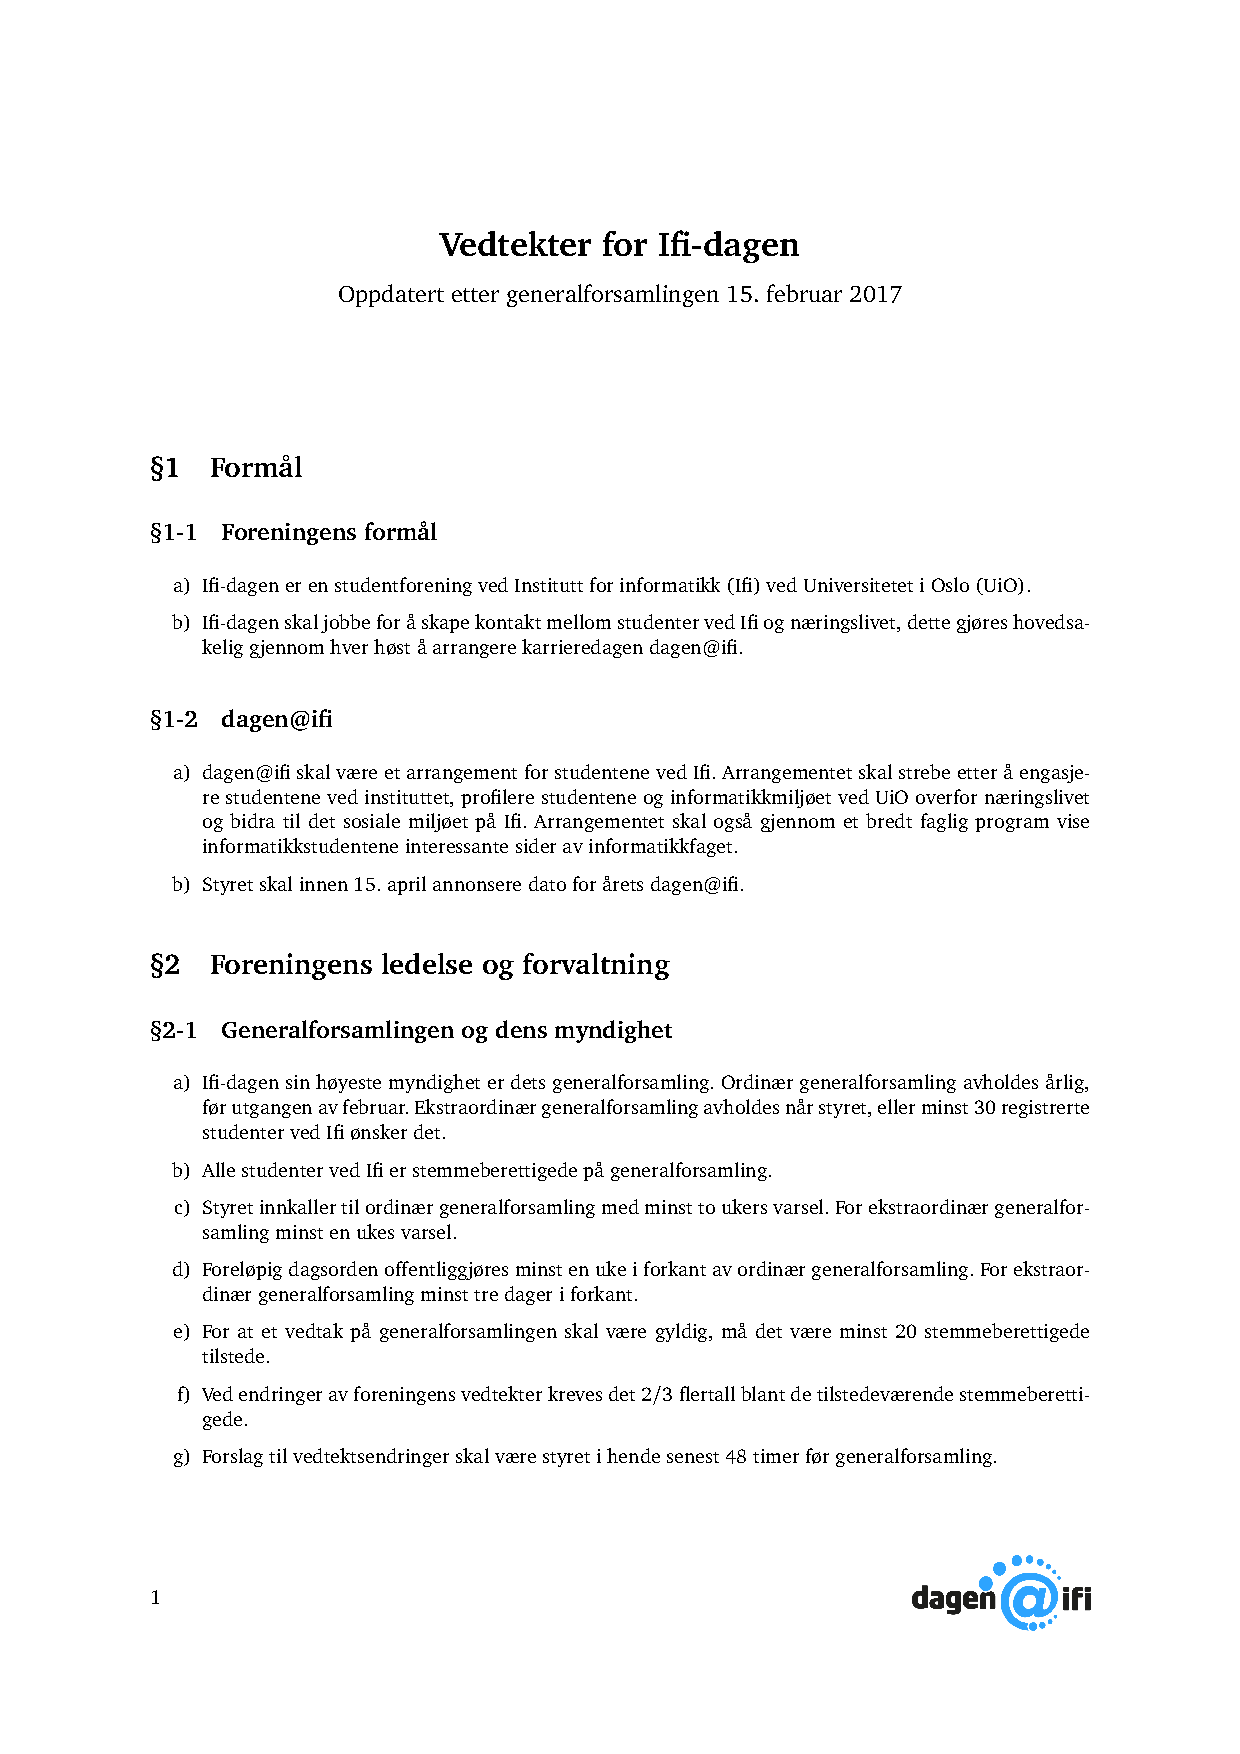
\includepdf[pages=-]{../vedtekter/vedtekter.pdf}
\end{document}
